\documentclass[12pt]{article}
\usepackage[T1]{fontenc}
\usepackage[T1]{polski}
\usepackage[utf8]{inputenc}
\newcommand{\BibTeX}{{\sc Bib}\TeX}
\usepackage{graphicx}
\usepackage{amsfonts}

% OWN PACKAGE - VERY IMPORTANT %
\usepackage{float}
%%%%%%%%%%%%%%%%%%%%%%%%%%%%%%%%%

\setlength{\textheight}{21cm}


\title{{\bf Zadanie nr 3 - Splot, filtracja i korelacja sygnałów}\linebreak
    Cyfrowe Przetwarzanie Sygnałów}
\author{Jan Karwowski 216793 \and Kamil Kowalewski 216806}
\date{data oddania zadania 29.04.2020r}

\begin{document}
    \clearpage\maketitle
    \thispagestyle{empty}
    \newpage
    \setcounter{page}{1}
%--------------------------------------------------------------------------------------%
    \section{Cel zadania} {
        Celem zadania jest zapoznanie się z operacjami splotu dyskretnego i korelacji
        dyskretnej, zaimplementowanie tychże operacji oraz wykorzystanie ich przy
        tworzeniu i zapoznaniu się z filtrami o skończonej odpowiedzi impulsowej.
    }
%--------------------------------------------------------------------------------------%
    \section{Wprowadzenie} {
        Operacja splotu jest jedną z podstawowych operacji wykorzystywanych w przetwarzaniu sygnałów
        cyfrowych. Polega ona na sumowaniu iloczynów próbek z dwóch sygnałów dysktretnych, aby
        otrzymać pojedynczą próbkę sygnału wynikowego. W przypadku sygnałów, którymi się
        posługujemy, czyli sygnałów o skończonej liczbie próbek indeksowanych od zera, operację
        splotu dwóch sygnałów dyskretncyh $x$ i $h$ przedstawia wzór:
        \begin{equation}
            (h \ast x)(n) = \sum_{k = 0}^{k = M - 1}h(k)x(n - k) \label{wzor:splot}
        \end{equation}
        Warto zwrócić uwagę, że jest to operacja przemienna, a liczba próbek sygnału wynikowego
        będzie wynosiła sumę liczb próbek sygnałów wejściowych mniej 1. Operacja ta została
        zaimplementowana w wynikowej aplikacji w ramach ralizacji omawianego zadania.

        Jednym z podstawowych zastosowań operacji splotu jest implementacja filtrów o skończonej
        odpowiedzi impulsowej. Filtry takie pozwalają zmienić widmo pewnego sygnału wejściowego $x$,
        poprzez wykonanie operacji splotu ze współczynnikami filtru $h$. Zgodnie ze znanym
        twierdzeniem o splocie, oznacza to wymnożenie widm filtru i sygnału wejściowego, a w wyniku
        daje sygnał, którego widmo jest "obcięte" w stosunku do sygnału filtrowanego - pewne
        częstotliwości składowe zostały wytłumione.  Wyróżniamy więc dla filtru pasmo zaporowe -
        częstotliwości składowe, które tłumimy, oraz pasmo przepustowe - częstotliwości składowe,
        które staramy się pozostawić niezmienione.  Wyróżniamy trzy rodzaje filtrów, wszystkie
        zostały zaimplementowane w ramach wykonywanego zadania. Pasma przepustowe i zaporowego
        każdego z nich są zależne od pewnego parametru filtru, nazywanego częstotliwością odcięcia
        $f_o$ oraz od częstotliwości próbkowania sygnału $f_p$. Przedstawione zakresy pasma
        przepustowego są charakterystyczne dla tego konretnego sposobu implementacji filtrów,
        opartego o filtr dolnoprzepustowy.
        \begin{itemize}
            \item filtr dolnoprzepustowy - pasmo przepustowe mieści się w zakresie od $0$ do $f_o$
            \item filtr górnoprzepustowy - pasmo przepustowe mieści się w zakresie od $f_p / 2 - f_o$ do
                $f_p / 2$
            \item filtr pasmowy - pasmo przepustowe mieście się w zakresie od $f_p / 4 - f_o$ do
                $f_p / 4 + f_o$
        \end{itemize}
        W praktyce taki filtr jest po prostu sygnałem dyskretnym $h$, którego długość nazywamy
        rzędem filtru $M$, wartości współczynników (próbek) nazywamy odpowiedzią impulsową, a widmo
        takiego sygnału nazywamy transmitancją filtru. Należy jeszcze wspomnieć, że idealny filtr
        miałby nieskończoną długość, natomiast ze względów praktycznych, rząd fitra zawsze jest
        skończony. Oznacza to, że z idealnego filtru "wycinamy" pewną skończoną liczbę próbek, co
        sprowadza się do wymnożenia odpowiedzi impulsowej filtru przez funkcję okna.
        Zaimplementowano cztery różne funkcje okna, które można wybrać podczas generowania filtru:
        \begin{itemize}
            \item okno prostokątne
            \item okno Hamminga
            \item okno Hanninga
            \item okno Blackmana
        \end{itemize}
        Każde z nich w inny sposób wpływa na zniekształcenie transmitancji idealnego filtru i może
        je zmniejszyć, tym samym poprawiając jakość filtrowania, lub zwiększyć, co przyczyni się do
        pogorszenia jakości filtrowania. W ramach wykonywanego zadania przygotowano możliwość
        generacji takich filtrów dla wybranych przez użytkownika parametrów. Aby następnie dokonać
        operacji filtrowania należy wykonać splot filtru $h$ z sygnałem $x$.

        Operacja korelacji sygnałów dyskretnych również jest jedną z podstawowych operacji
        wykorzystywanych podczas cyfrowego przetwarzania sygnałów. Przypomina operację splotu, a
        nawet może być zaimplementowana na jego podstawie. Dla skończonych sygnałów dyskretnych $x$
        oraz $h$, które są indeksowane od zera, operacja ta jest reprezentowana wzorem:
        \begin{equation}
            R_{hx} = \sum_{k = 0}^{M - 1}h(k)x(k - n) \label{wzor:korelacja}
        \end{equation}
        Widać, że wzory te są bardzo podobne, co będzie skutkowało pewnym podobieństwem korelacji i
        splotu tych samych dwóch sygnałów dyskretnych. W ramach realizacji zadania operacja ta
        została zaimplementowana w tworzonej aplikacji.

        Aby przedstawić zastosowanie analizy korelacyjnej sygnałów, zaimplementowano również
        symulator korelacyjnego czujnika odległości. Działania takiego urządzenia jest bardzo
        proste i opiera się o pomiar opóźnienia sygnału powrotnego (odbitego od obiektu) w
        stosunku do sygnału sondującego (wysłanego w kierunku obiektu) z wykorzystaniem korelacji
        wspomnianych sygnałów. Jeżeli takie opóźnienie jest mniejsze niż okres sygnału sondującego,
        to w zależności od częstotliwości próbkowania, można mniej lub bardziej precyzyjnie określić
        odległość od obiektu, wykorzystując oczywiście podstawy wzór na zależność drogi od czasu,
        przy stałej prędkości:
        \begin{equation}
            S = V \cdot t \label{wzor:droga}
        \end{equation}
        Pomiar opóźnienia opiera się o założenie, że korelacja sygnałów jest największa, kiedy
        sygnały te są takie same (idealnie nakładają się na siebie). Sygnał będący wynikiem
        korelacji zawiera właśnie wyniki nałożenia na siebie dwóch sygnałów w odstępach czasu
        równych okresowi próbkowania. Wystarczy więc znaleźć maksimum korelacji (licząc od środkowej
        próbki w prawo) aby okreslić, jakie jest opóźnienie sygnału zwrotnego.
    }
%--------------------------------------------------------------------------------------%
    \section{Materiały i metody} {

        \subsection{Splot i korelacja sygnałów dyskretnych} {
            Pojedynczy eksperyment składał się z kilku kroków. Najpierw wygenerowano wybrane sygnały
            ciągłe (wykorzystano funkcję sin, kwadratową i trójkątną), następnie spróbkowano je z
            ustaloną częstotliwości i na wynikach próbkowania przeprowadzono operację splotu lub
            korelacji.
            Skróty w tabelach oznaczają kolejno:
            \begin{itemize}
                \item Amplituda: Ampl
                \item Czas początkowy: Czas pocz
                \item Czas trwania sygnału: Czas trw syg
                \item Okres podstawowy: Okres pods
                \item Współczynnik wypełnienia: Współ wypeł
                \item Częstotliwość próbkowania: Częs próbk
            \end{itemize}
        }

        \subsection{Filtracja sygnałów dyskretnych} \label{metody:filtracja}{
            W każdym eksperymencie mającym na celu prezentację procesu filtrowania wykorzystany
            został inny filtr, który uprzednio wygenerowano wykorzystując wybrane parametry. Sygnał
            filtrowany natomiast wykorzystano ten sam, dla wszystkich eksperymentów. Jest to
            suma dwóch sygnałów sinusoidalnych $s_1$ i $s_2$ o następujących parametrach:
            \begin{itemize}
                \item częstotliwość $f_{s_1} = 3Hz$
                \item amplituda $A_{s_1} = 2$
                \item częstotliwość $f_{s_2} = 20Hz$
                \item amplituda $A_{s_2} = 0.5$
                \item czas trwania $1s$
                \item częstotliwość próbkowania $f_s = 400Hz$
            \end{itemize}
            \begin{figure}[H]
                \centering
                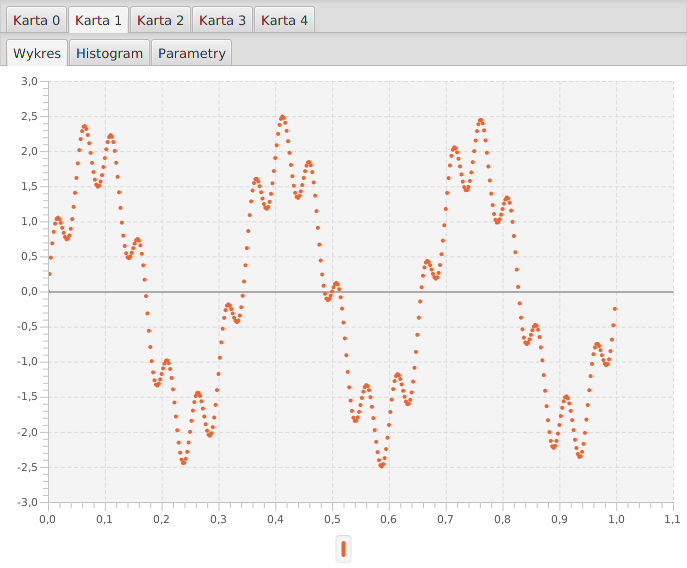
\includegraphics[width=0.7\textwidth]{img/result/filter/filtered.png}
                \caption{Sygnał filtrowany} \label{wykres:filtrowany}
            \end{figure}
            Każdorazowo po wygenerowaniu filtru obliczony został jego splot z sygnałem
            filtrowanym. Dla każdego eksperymentu zaprezentowano parametry i typ generowanego
            filtru, sam filtr oraz wynik splotu. W przypadku niektórych eksperymentów wykonano
            rekonstrukcję wyniku filtrowania (interpolację pierwszego rzędu), w celu zwiększenia
            przejrzystości wyniku.
        }

        \subsection{Wykorzystanie analizy korelacyjnej do pomiaru odległości} {
            W przypadku wykorzystania analizy korelacyjnej do pomiaru odległości wykorzystano
            niezależną funkcjonalność aplikacji, jaką jest symulator korelacyjnego czujnika
            odległości. Każdy eksperyment wykonany został poprzez jednokrotne uruchomienie
            symulatora. Udokumentowane zostały parametry wejściowe i parametry wyjściowe z
            kilku chwil czasu. Wykorzystane zostały następujące oznaczenia parametrów
            wejściowych:
            \begin{itemize}
                \item $V_s[m/s]$ - prędkość sygnału w ośrodku
                \item $V_p[m/s]$ - prędkość przedmiotu
                \item $T_s[s]$ - okres sygnału sondującego
                \item $f_s[Hz]$ - częstotliwość próbkowania czujnika odległości
                \item $l$ - długość bufora czujnika odległości
            \end{itemize}
            Okres raportowania zawsze był ustawiony na $0.5s$ a jedna jenostka czasu w
            symulatorze na $0.1s$. Początkowy dystans do przedmiotu wynosi $25m$.
            Wykorzystane zostały następujące oznaczenia parametrów wyjściowych:
            \begin{itemize}
                \item $t[s]$ - chwila czasu
                \item $d_r[m]$ - odległość rzeczywista do przedmiotu
                \item $d_m[s]$ - odległość obliczona przez czujnik odległości
            \end{itemize}
        }
    }
    \newpage
%--------------------------------------------------------------------------------------%
    \section{Eksperymenty i wyniki} {

        \subsection{Splot i korelacja sygnałów dyskretnych} {

            \subsubsection{Splot sygnałów sinusoidalnych} \label{eksperyment:splot1}{

                \begin{table}[H]
                    \centering
                    \begin{tabular}{|l|l|l|l|l|}
                        \hline
                        Ampl & Czas pocz & Czas trw syg & Okres pods & Częs próbk   \\ \hline
                        1 & 0s & 3s & 1 & 100           \\ \hline
                    \end{tabular}
                    \caption{Parametry wejściowe dla sygnału nr 1}
                \end{table}
                \begin{figure}[H]
                    \centering
                    \includegraphics[width=0.7\textwidth]{img/result/convolution/experiment1/data_105849.png}
                    \caption{Wykres sygnału numer 1}
                \end{figure}

                \begin{table}[H]
                    \centering
                    \begin{tabular}{|l|l|l|l|l|}
                        \hline
                        Ampl & Czas pocz & Czas trw syg & Okres pods & Częs próbk   \\ \hline
                        1 & 2s & 3s & 1 & 100           \\ \hline
                    \end{tabular}
                    \caption{Parametry wejściowe dla sygnału nr 2}
                \end{table}
                \begin{figure}[H]
                    \centering
                    \includegraphics[width=0.7\textwidth]{img/result/convolution/experiment1/data_105856.png}
                    \caption{Wykres sygnału numer 2}
                \end{figure}

                \begin{figure}[H]
                    \centering
                    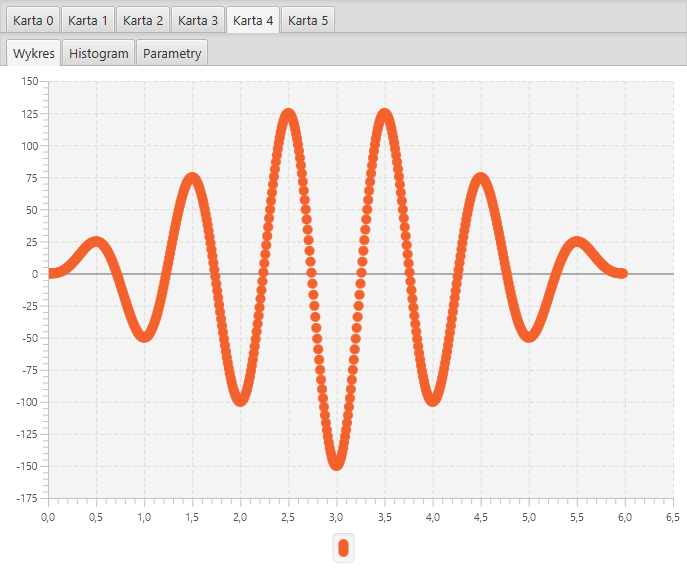
\includegraphics[width=0.9\textwidth]{img/result/convolution/experiment1/data_105901.png}
                    \caption{Wykres sygnału po operacji splotu}
                \end{figure}
            }
            \newpage

            \subsubsection{Splot sygnałów sinsoidalnego oraz sinusoidalnego wyprostowanego
            jednopołówkowo} \label{eksperyment:splot2}{

                \begin{table}[H]
                    \centering
                    \begin{tabular}{|l|l|l|l|l|}
                        \hline
                        Ampl & Czas pocz & Czas trw syg & Okres pods & Częs próbk   \\ \hline
                        1 & 0s & 3s & 1 & 100           \\ \hline
                    \end{tabular}
                    \caption{Parametry wejściowe dla sygnału nr 1}
                \end{table}
                \begin{figure}[H]
                    \centering
                    \includegraphics[width=0.7\textwidth]{img/result/convolution/experiment2/data_122746.png}
                    \caption{Wykres sygnału numer 1}
                \end{figure}

                \begin{table}[H]
                    \centering
                    \begin{tabular}{|l|l|l|l|l|}
                        \hline
                        Ampl & Czas pocz & Czas trw syg & Okres pods & Częs próbk   \\ \hline
                        2 & 1s & 3s & 1 & 100           \\ \hline
                    \end{tabular}
                    \caption{Parametry wejściowe dla sygnału nr 2}
                \end{table}
                \begin{figure}[H]
                    \centering
                    \includegraphics[width=0.7\textwidth]{img/result/convolution/experiment2/data_122752.png}
                    \caption{Wykres sygnału numer 2}
                \end{figure}

                \begin{figure}[H]
                    \centering
                    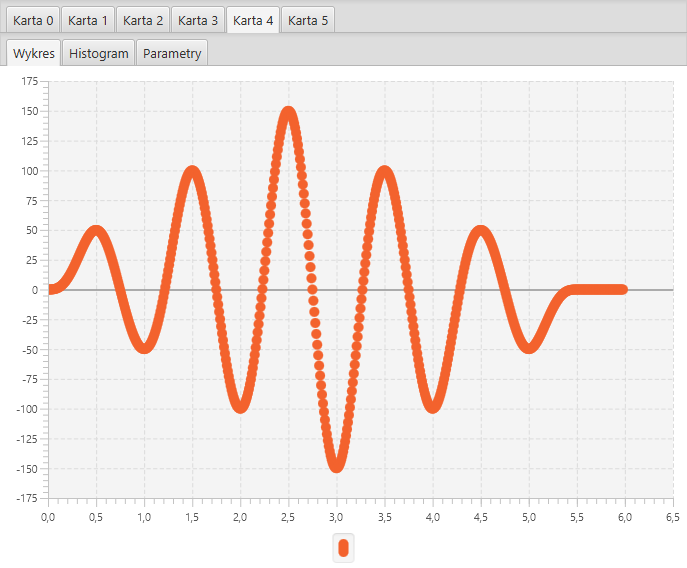
\includegraphics[width=0.9\textwidth]{img/result/convolution/experiment2/data_122802.png}
                    \caption{Wykres sygnału po operacji splotu}
                \end{figure}
            }
            \newpage

            \subsubsection{Splot sygnałów sinusoidalnego oraz trójkątnego} \label{eksperyment:splot3}{

                \begin{table}[H]
                    \centering
                    \begin{tabular}{|l|l|l|l|l|}
                        \hline
                        Ampl & Czas pocz & Czas trw syg & Okres pods & Częs próbk   \\ \hline
                        1 & 0s & 3s & 1 & 100           \\ \hline
                    \end{tabular}
                    \caption{Parametry wejściowe dla sygnału nr 1}
                \end{table}
                \begin{figure}[H]
                    \centering
                    \includegraphics[width=0.7\textwidth]{img/result/convolution/experiment3/data_124714.png}
                    \caption{Wykres sygnału numer 1}
                \end{figure}

                \begin{table}[H]
                    \centering
                    \begin{tabular}{|l|l|l|l|l|l|}
                        \hline
                        Ampl & Czas pocz & Czas trw syg & Okres pods & Współ wypeł & Częs próbk   \\\hline
                        2 & 1s & 3s & 0.5 & 0.5 & 70           \\\hline
                    \end{tabular}
                    \caption{Parametry wejściowe dla sygnału nr 2}
                \end{table}
                \begin{figure}[H]
                    \centering
                    \includegraphics[width=0.7\textwidth]{img/result/convolution/experiment3/data_124722.png}
                    \caption{Wykres sygnału numer 2}
                \end{figure}

                \begin{figure}[H]
                    \centering
                    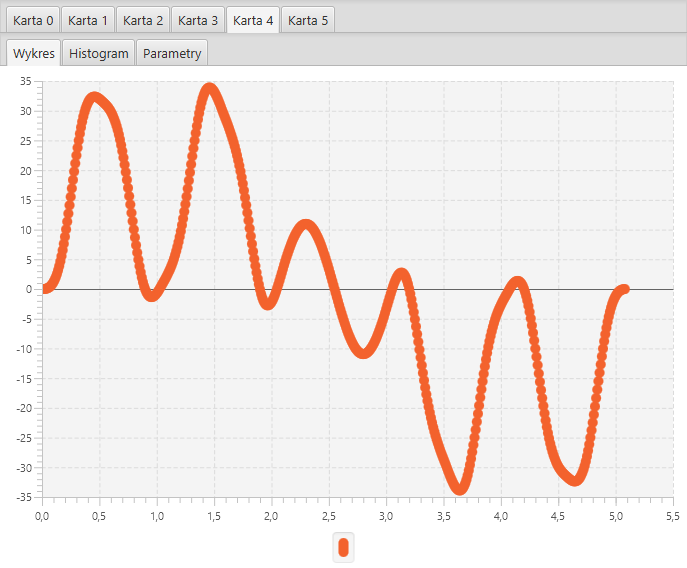
\includegraphics[width=0.9\textwidth]{img/result/convolution/experiment3/data_124733.png}
                    \caption{Wykres sygnału po operacji splotu}
                \end{figure}
            }
            \newpage

            \subsubsection{Korelacja sygnałów sinusoidalnych} \label{eksperyment:korelacja1}{

                \begin{table}[H]
                    \centering
                    \begin{tabular}{|l|l|l|l|l|}
                        \hline
                        Ampl & Czas pocz & Czas trw syg & Okres pods & Częs próbk   \\ \hline
                        1 & 0s & 3s & 1 & 100           \\ \hline
                    \end{tabular}
                    \caption{Parametry wejściowe dla sygnału nr 1}
                \end{table}
                \begin{figure}[H]
                    \centering
                    \includegraphics[width=0.7\textwidth]{img/result/correlation/experiment1/data_105849.png}
                    \caption{Wykres sygnału numer 1}
                \end{figure}

                \begin{table}[H]
                    \centering
                    \begin{tabular}{|l|l|l|l|l|}
                        \hline
                        Ampl & Czas pocz & Czas trw syg & Okres pods & Częs próbk   \\ \hline
                        1 & 2s & 3s & 1 & 100           \\ \hline
                    \end{tabular}
                    \caption{Parametry wejściowe dla sygnału nr 2}
                \end{table}
                \begin{figure}[H]
                    \centering
                    \includegraphics[width=0.7\textwidth]{img/result/correlation/experiment1/data_105856.png}
                    \caption{Wykres sygnału numer 2}
                \end{figure}

                \begin{figure}[H]
                    \centering
                    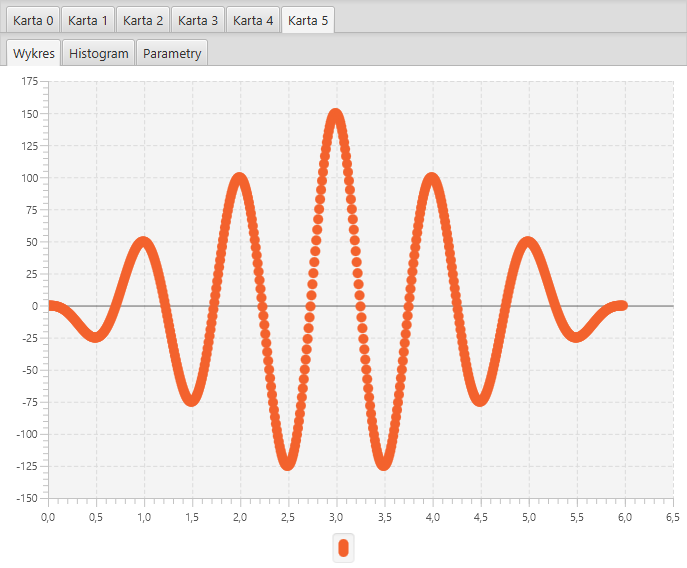
\includegraphics[width=0.9\textwidth]{img/result/correlation/experiment1/data_105906.png}
                    \caption{Wykres sygnału po operacji korelacji}
                \end{figure}
            }
            \newpage

            \subsubsection{Korelacja sygnałów sinusoidalnego z sinusoidalnym wyprostowanym
            jednopołówkowo} \label{eksperyment:korelacja2}{

                \begin{table}[H]
                    \centering
                    \begin{tabular}{|l|l|l|l|l|}
                        \hline
                        Ampl & Czas pocz & Czas trw syg & Okres pods & Częs próbk   \\ \hline
                        1 & 0s & 3s & 1 & 100           \\ \hline
                    \end{tabular}
                    \caption{Parametry wejściowe dla sygnału nr 1}
                \end{table}
                \begin{figure}[H]
                    \centering
                    \includegraphics[width=0.7\textwidth]{img/result/correlation/experiment2/data_122746.png}
                    \caption{Wykres sygnału numer 1}
                \end{figure}

                \begin{table}[H]
                    \centering
                    \begin{tabular}{|l|l|l|l|l|}
                        \hline
                        Ampl & Czas pocz & Czas trw syg & Okres pods & Częs próbk   \\ \hline
                        2 & 1s & 3s & 1 & 100           \\ \hline
                    \end{tabular}
                    \caption{Parametry wejściowe dla sygnału nr 2}
                \end{table}
                \begin{figure}[H]
                    \centering
                    \includegraphics[width=0.7\textwidth]{img/result/correlation/experiment2/data_122752.png}
                    \caption{Wykres sygnału numer 2}
                \end{figure}

                \begin{figure}[H]
                    \centering
                    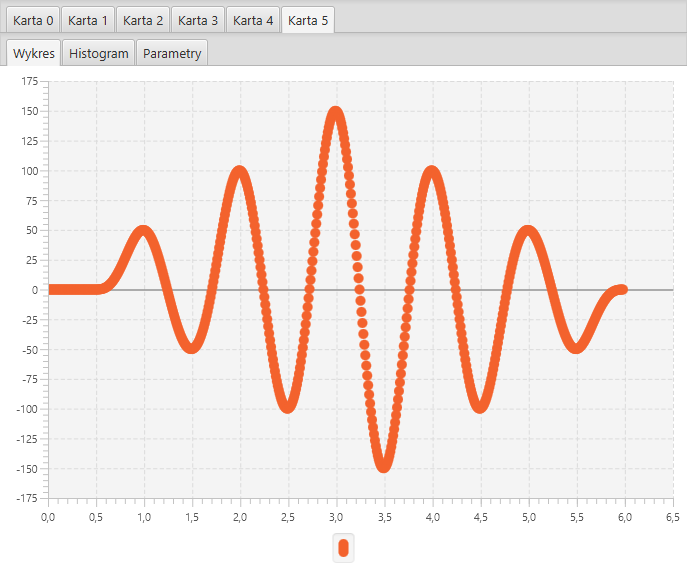
\includegraphics[width=0.9\textwidth]{img/result/correlation/experiment2/data_122807.png}
                    \caption{Wykres sygnału po operacji korelacji}
                \end{figure}
            }
            \newpage

            \subsubsection{Korelacja sygnałów sinusoidalnego oraz trójkątnego} \label{eksperyment:korelacja3}{

                \begin{table}[H]
                    \centering
                    \begin{tabular}{|l|l|l|l|l|}
                        \hline
                        Ampl & Czas pocz & Czas trw syg & Okres pods & Częs próbk   \\\hline
                        1 & 0s & 3s & 1 & 100           \\\hline
                    \end{tabular}
                    \caption{Parametry wejściowe dla sygnału nr 1}
                \end{table}
                \begin{figure}[H]
                    \centering
                    \includegraphics[width=0.7\textwidth]{img/result/correlation/experiment3/data_124714.png}
                    \caption{Wykres sygnału numer 1}
                \end{figure}

                \begin{table}[H]
                    \centering
                    \begin{tabular}{|l|l|l|l|l|l|}
                        \hline
                        Ampl & Czas pocz & Czas trw syg & Okres pods & Współ wypeł & Częs próbk   \\\hline
                        2 & 1s & 3s & 0.5 & 0.5 & 70     \\\hline
                    \end{tabular}
                    \caption{Parametry wejściowe dla sygnału nr 2}
                \end{table}
                \begin{figure}[H]
                    \centering
                    \includegraphics[width=0.7\textwidth]{img/result/correlation/experiment3/data_124722.png}
                    \caption{Wykres sygnału numer 2}
                \end{figure}

                \begin{figure}[H]
                    \centering
                    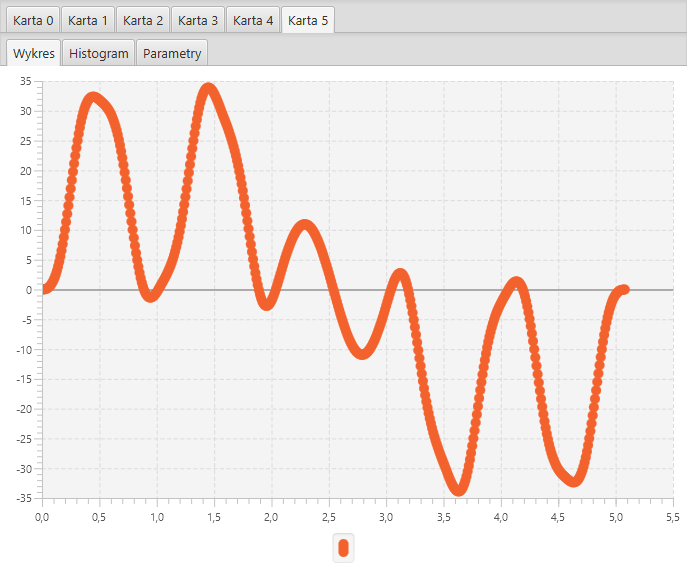
\includegraphics[width=0.9\textwidth]{img/result/correlation/experiment3/data_124738.png}
                    \caption{Wykres sygnału po operacji korelacji}
                \end{figure}
            }
            \newpage
        }
%--------------------------------------------------------------------------------------%
        \subsection{Filtracja sygnałów dyskretnych} {

            \subsubsection{Eksperyment 1} {
                \begin{table}[H]
                \centering
                \begin{tabular}{|l|l|l|l|l|l|}
                \hline
                Typ filtra & Rząd filtra & Częstotliwość odcięcia & Typ okna  \\\hline
                low\_pass & 51 & 5 & rectangular     \\\hline
                \end{tabular}
                \caption{Parametry filtra}
                \end{table}
                \begin{figure}[H]
                \centering
                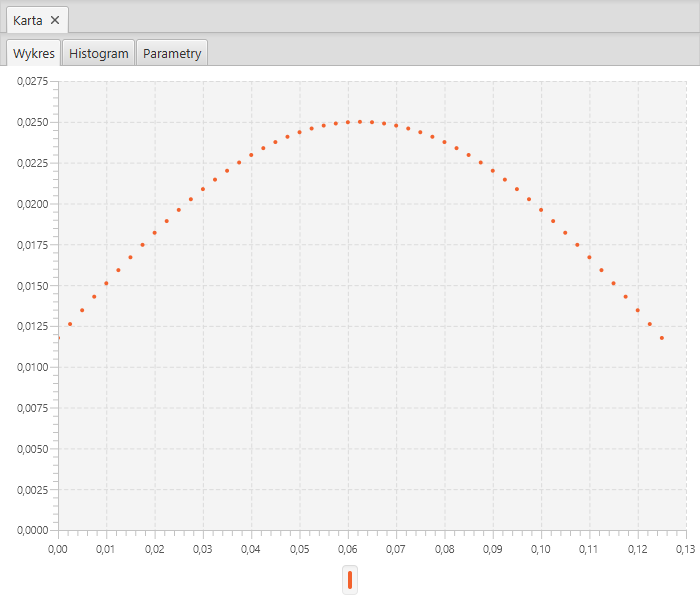
\includegraphics[width=0.55\textwidth]{img/result/filter/experiment01/data_draw_1a_filter_data_115323.png}
                \caption{Wykres filtra}
                \end{figure}

                \begin{figure}[H]
                \centering
                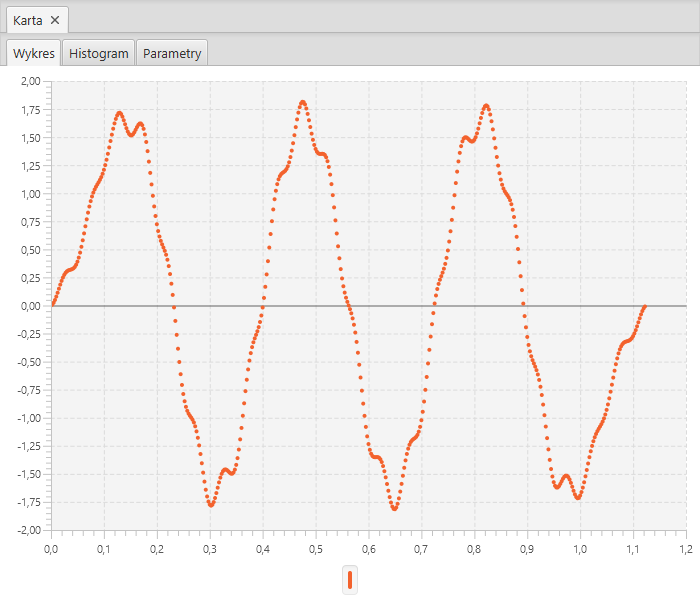
\includegraphics[width=0.55\textwidth]{img/result/filter/experiment01/data_draw_1a_result_data_115329.png}
                \caption{Wykres sygnału po filtracji}
                \end{figure}
            }
            \newpage

            \subsubsection{Eksperyment 2} {
                \begin{table}[H]
                \centering
                \begin{tabular}{|l|l|l|l|l|l|}
                \hline
                Typ filtra & Rząd filtra & Częstotliwość odciecia & Typ okna  \\\hline
                low\_pass & 51 & 5 & hamming     \\\hline
                \end{tabular}
                \caption{Parametry filtra}
                \end{table}
                \begin{figure}[H]
                \centering
                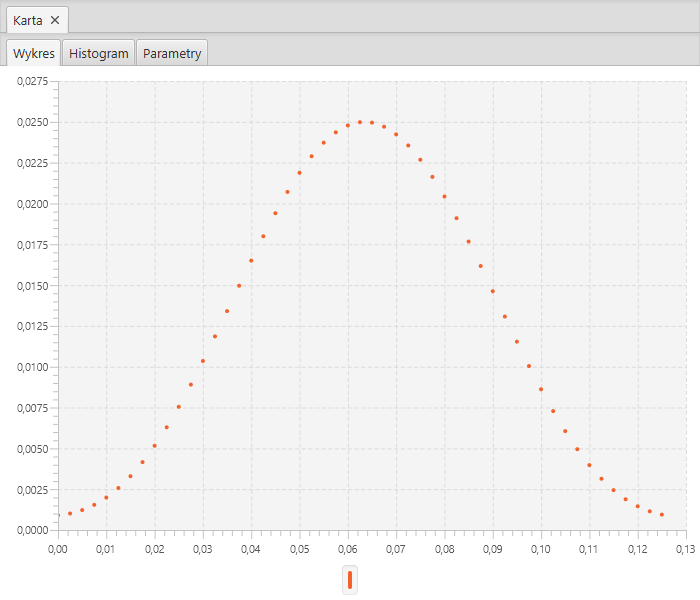
\includegraphics[width=0.6\textwidth]{img/result/filter/experiment02/data_draw_1b_filter_data_113443.png}
                \caption{Wykres filtra}
                \end{figure}

                \begin{figure}[H]
                \centering
                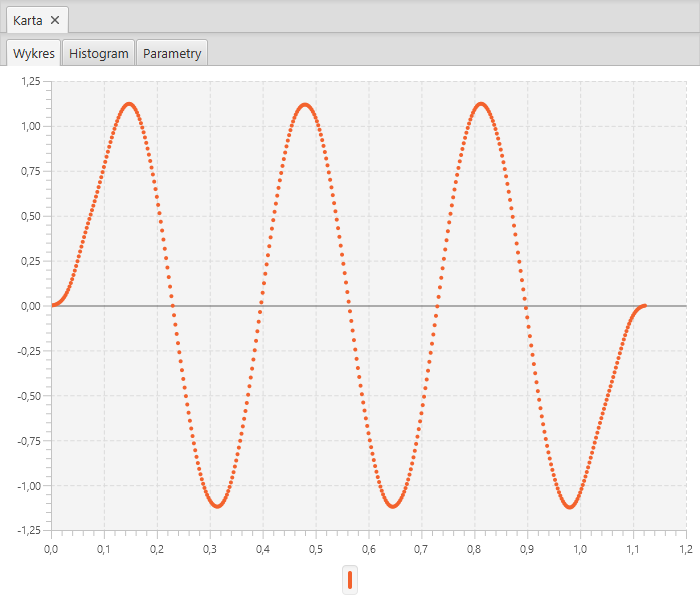
\includegraphics[width=0.6\textwidth]{img/result/filter/experiment02/data_draw_1b_result_data_113446.png}
                \caption{Wykres sygnału po filtracji}
                \end{figure}
            }
            \newpage

            \subsubsection{Eksperyment 3} {
                \begin{table}[H]
                \centering
                \begin{tabular}{|l|l|l|l|l|l|}
                \hline
                Typ filtra & Rząd filtra & Częstotliwość odciecia & Typ okna  \\\hline
                low\_pass & 51 & 5 & hanning     \\\hline
                \end{tabular}
                \caption{Parametry filtra}
                \end{table}
                \begin{figure}[H]
                \centering
                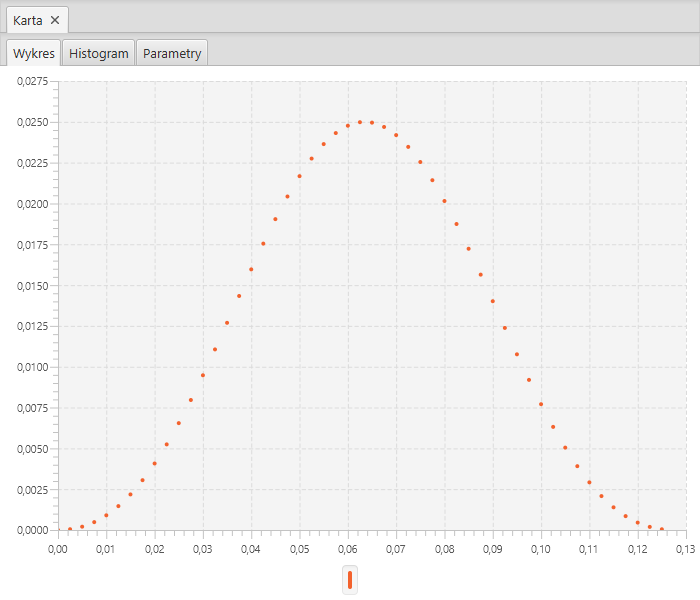
\includegraphics[width=0.6\textwidth]{img/result/filter/experiment03/data_draw_1c_filter_data_113451.png}
                \caption{Wykres filtra}
                \end{figure}

                \begin{figure}[H]
                \centering
                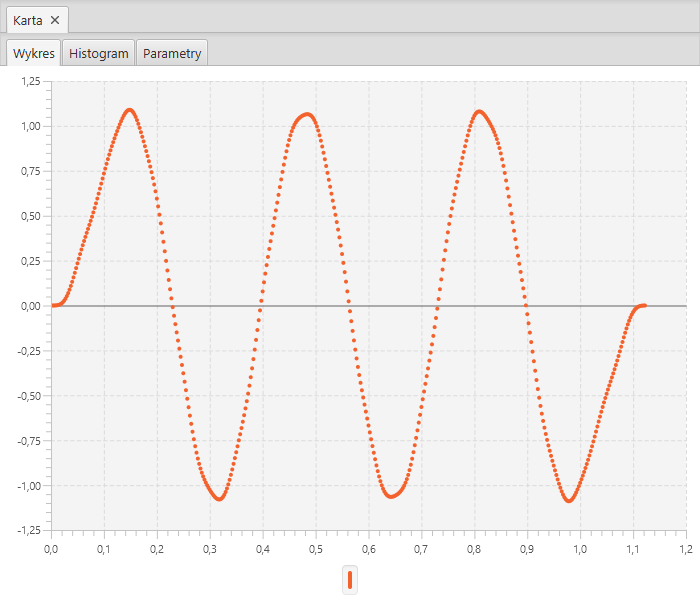
\includegraphics[width=0.6\textwidth]{img/result/filter/experiment03/data_draw_1c_result_data_113455.png}
                \caption{Wykres sygnału po filtracji}
                \end{figure}
            }
            \newpage

            \subsubsection{Eksperyment 4} {
                \begin{table}[H]
                \centering
                \begin{tabular}{|l|l|l|l|l|l|}
                \hline
                Typ filtra & Rząd filtra & Częstotliwość odciecia & Typ okna  \\\hline
                low\_pass & 51 & 5 & blackman     \\\hline
                \end{tabular}
                \caption{Parametry filtra}
                \end{table}
                \begin{figure}[H]
                \centering
                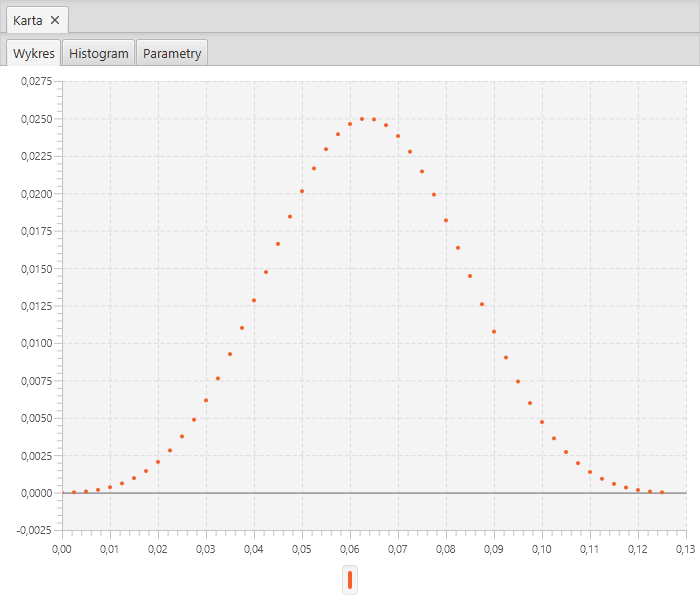
\includegraphics[width=0.6\textwidth]{img/result/filter/experiment04/data_draw_1d_filter_data_113501.png}
                \caption{Wykres filtra}
                \end{figure}

                \begin{figure}[H]
                \centering
                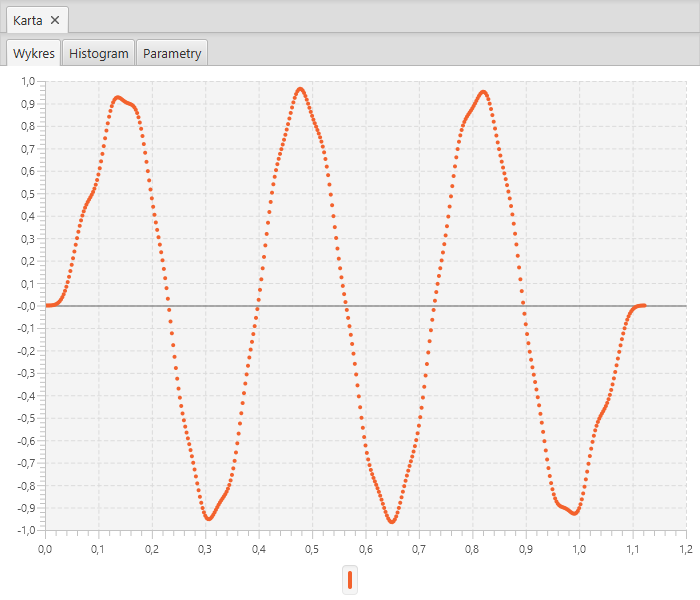
\includegraphics[width=0.6\textwidth]{img/result/filter/experiment04/data_draw_1d_result_data_113504.png}
                \caption{Wykres sygnału po filtracji}
                \end{figure}
            }
            \newpage

            \subsubsection{Eksperyment 5} {
                \begin{table}[H]
                \centering
                \begin{tabular}{|l|l|l|l|l|l|}
                \hline
                Typ filtra & Rząd filtra & Częstotliwość odciecia & Typ okna  \\\hline
                low\_pass & 41 & 5 & hamming     \\\hline
                \end{tabular}
                \caption{Parametry filtra}
                \end{table}
                \begin{figure}[H]
                \centering
                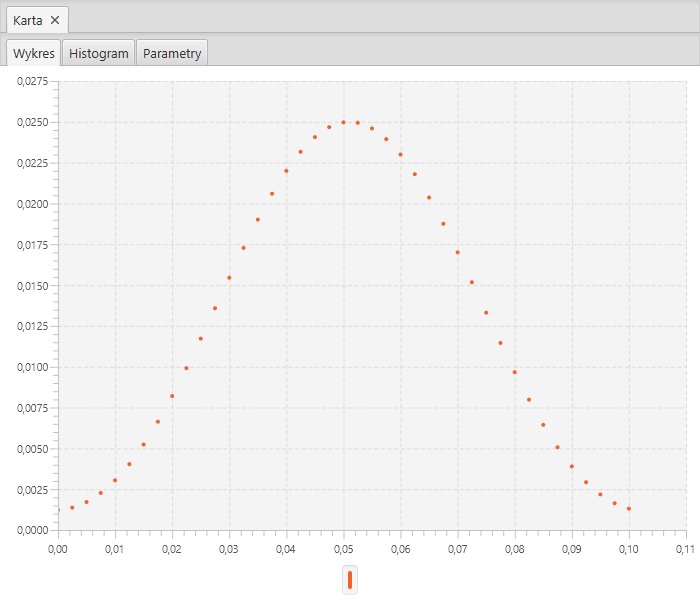
\includegraphics[width=0.6\textwidth]{img/result/filter/experiment05/data_draw_2a_filter_data_114000.png}
                \caption{Wykres filtra}
                \end{figure}

                \begin{figure}[H]
                \centering
                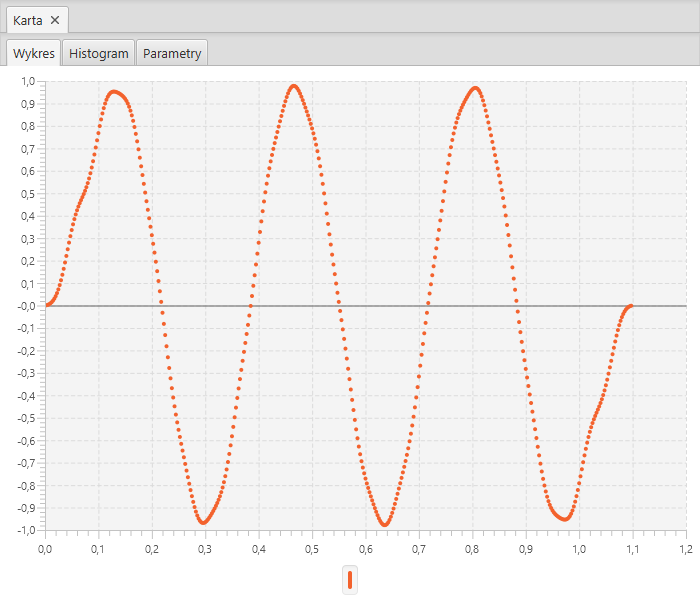
\includegraphics[width=0.6\textwidth]{img/result/filter/experiment05/data_draw_2a_result_data_114003.png}
                \caption{Wykres sygnału po filtracji}
                \end{figure}
            }
            \newpage

            \subsubsection{Eksperyment 6} {
                \begin{table}[H]
                \centering
                \begin{tabular}{|l|l|l|l|l|l|}
                \hline
                Typ filtra & Rząd filtra & Częstotliwość odciecia & Typ okna  \\\hline
                low\_pass & 31 & 5 & hamming     \\\hline
                \end{tabular}
                \caption{Parametry filtra}
                \end{table}
                \begin{figure}[H]
                \centering
                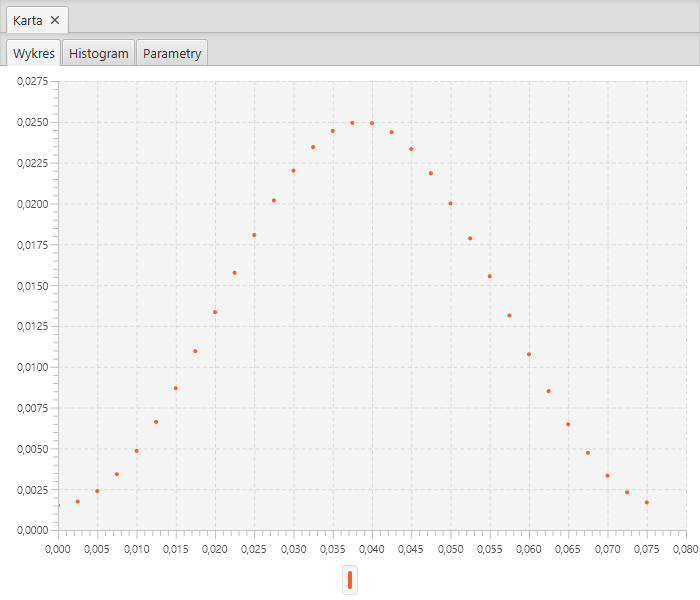
\includegraphics[width=0.6\textwidth]{img/result/filter/experiment06/data_draw_2b_filter_data_114016.png}
                \caption{Wykres filtra}
                \end{figure}

                \begin{figure}[H]
                \centering
                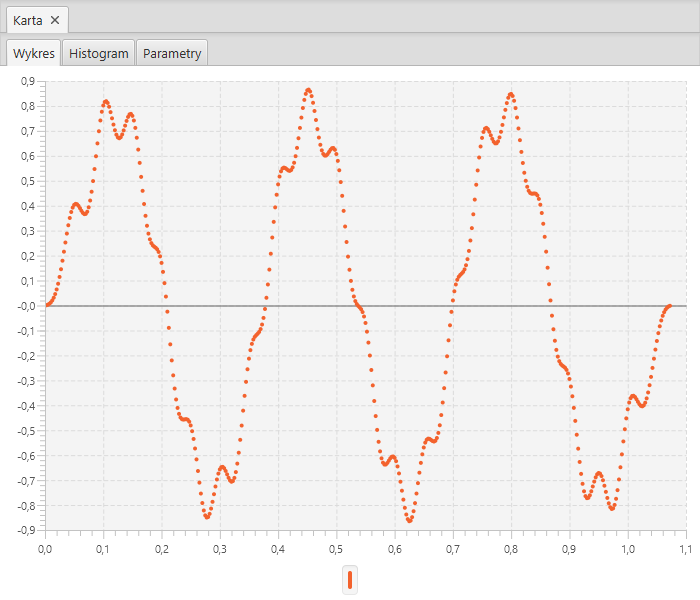
\includegraphics[width=0.6\textwidth]{img/result/filter/experiment06/data_draw_2b_result_data_114019.png}
                \caption{Wykres sygnału po filtracji}
                \end{figure}
            }
            \newpage

            \subsubsection{Eksperyment 7} {
                \begin{table}[H]
                \centering
                \begin{tabular}{|l|l|l|l|l|l|}
                \hline
                Typ filtra & Rząd filtra & Częstotliwość odciecia & Typ okna  \\\hline
                low\_pass & 21 & 5 & hamming     \\\hline
                \end{tabular}
                \caption{Parametry filtra}
                \end{table}
                \begin{figure}[H]
                \centering
                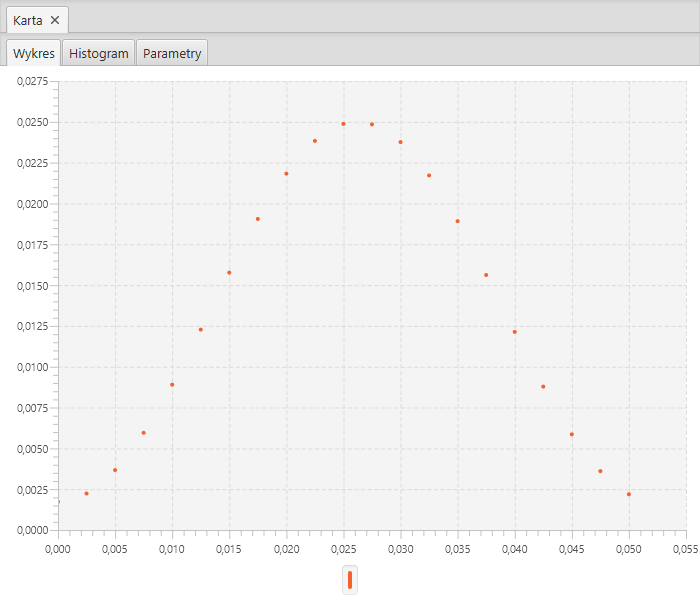
\includegraphics[width=0.6\textwidth]{img/result/filter/experiment07/data_draw_2c_filter_data_114026.png}
                \caption{Wykres filtra}
                \end{figure}

                \begin{figure}[H]
                \centering
                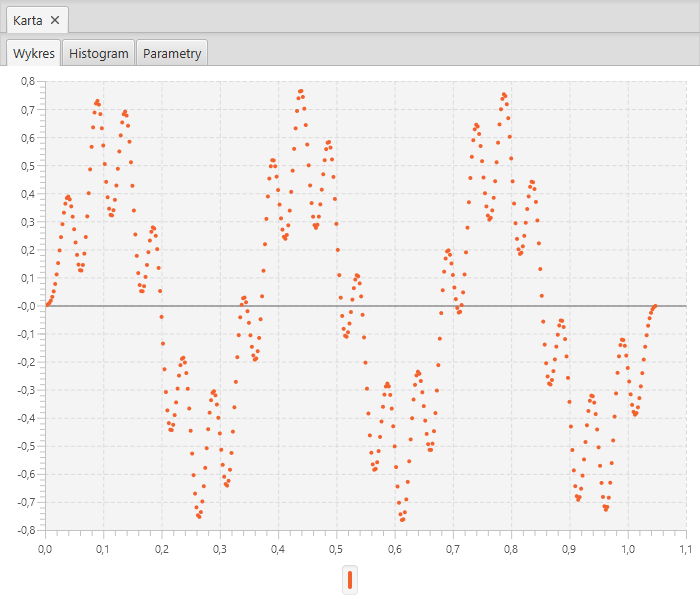
\includegraphics[width=0.6\textwidth]{img/result/filter/experiment07/data_draw_2c_result_data_114030.png}
                \caption{Wykres sygnału po filtracji}
                \end{figure}
            }
            \newpage

            \subsubsection{Eksperyment 8} {
                \begin{table}[H]
                \centering
                \begin{tabular}{|l|l|l|l|l|l|}
                \hline
                Typ filtra & Rząd filtra & Częstotliwość odciecia & Typ okna  \\\hline
                low\_pass & 51 & 3 & hamming     \\\hline
                \end{tabular}
                \caption{Parametry filtra}
                \end{table}
                \begin{figure}[H]
                \centering
                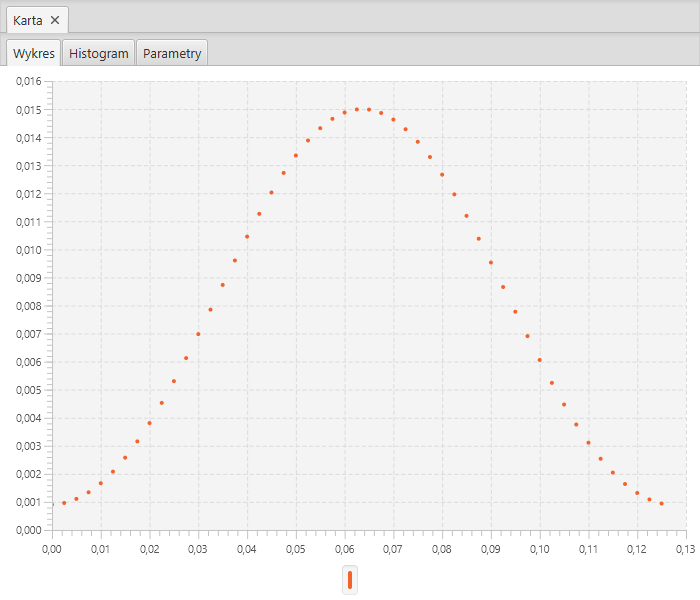
\includegraphics[width=0.6\textwidth]{img/result/filter/experiment08/data_draw_3a_filter_data_114037.png}
                \caption{Wykres filtra}
                \end{figure}

                \begin{figure}[H]
                \centering
                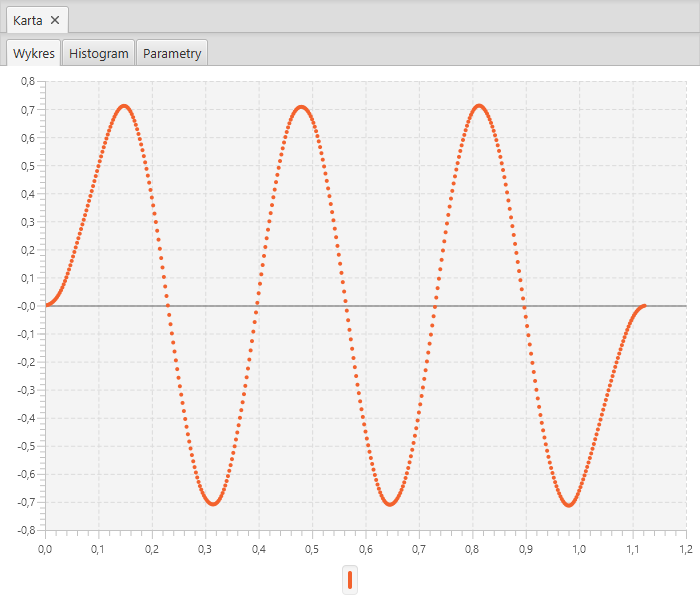
\includegraphics[width=0.6\textwidth]{img/result/filter/experiment08/data_draw_3a_result_data_114041.png}
                \caption{Wykres sygnału po filtracji}
                \end{figure}
            }
            \newpage

            \subsubsection{Eksperyment 9} {
                \begin{table}[H]
                \centering
                \begin{tabular}{|l|l|l|l|l|l|}
                \hline
                Typ filtra & Rząd filtra & Częstotliwość odciecia & Typ okna  \\\hline
                low\_pass & 51 & 2 & hamming     \\\hline
                \end{tabular}
                \caption{Parametry filtra}
                \end{table}
                \begin{figure}[H]
                \centering
                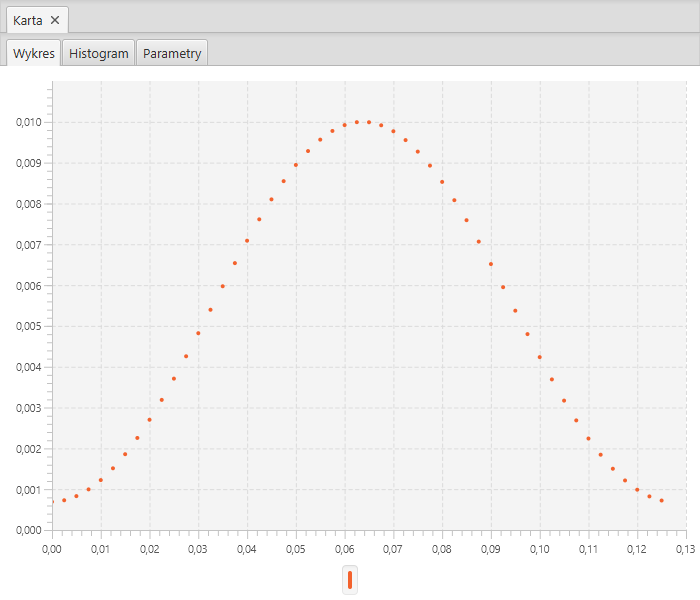
\includegraphics[width=0.6\textwidth]{img/result/filter/experiment09/data_draw_3b_filter_data_114048.png}
                \caption{Wykres filtra}
                \end{figure}

                \begin{figure}[H]
                \centering
                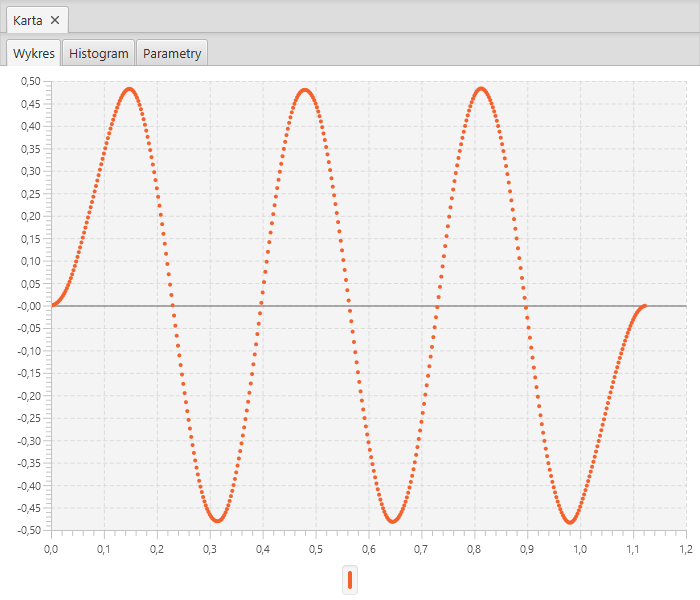
\includegraphics[width=0.6\textwidth]{img/result/filter/experiment09/data_draw_3b_result_data_114051.png}
                \caption{Wykres sygnału po filtracji}
                \end{figure}
            }
            \newpage

            \subsubsection{Eksperyment 10} {
                \begin{table}[H]
                \centering
                \begin{tabular}{|l|l|l|l|l|l|}
                \hline
                Typ filtra & Rząd filtra & Częstotliwość odciecia & Typ okna  \\\hline
                high\_pass & 51 & 190 & hamming     \\\hline
                \end{tabular}
                \caption{Parametry filtra}
                \end{table}
                \begin{figure}[H]
                \centering
                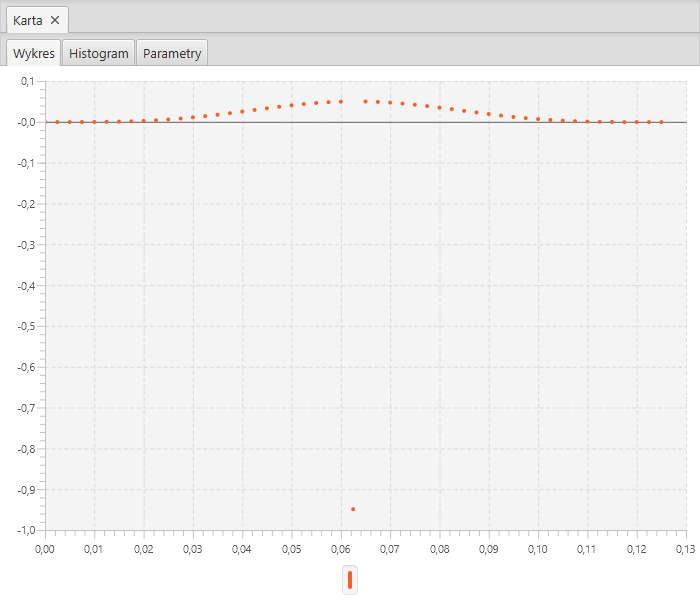
\includegraphics[width=0.6\textwidth]{img/result/filter/experiment10/data_draw_3c_filter_data_114057.png}
                \caption{Wykres filtra}
                \end{figure}

                \begin{figure}[H]
                \centering
                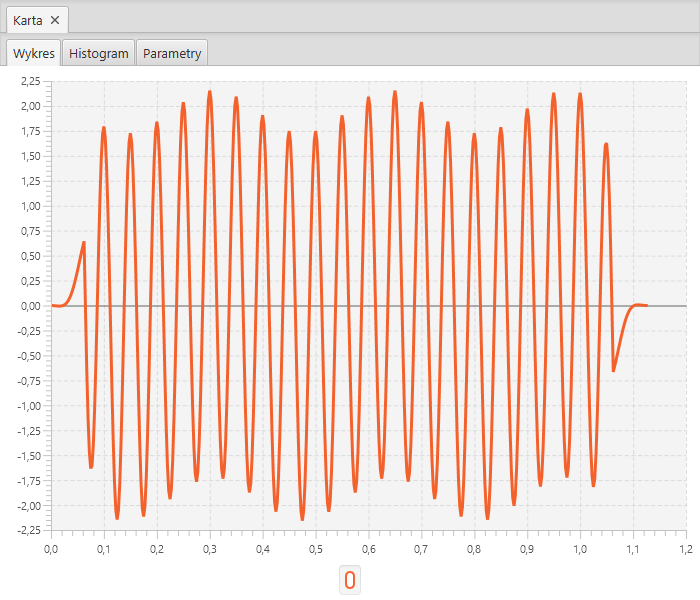
\includegraphics[width=0.6\textwidth]{img/result/filter/experiment10/data_draw_3c_result_reconstr_data_114200.png}
                \caption{Wykres sygnału po filtracji}
                \end{figure}
            }
            \newpage

            \subsubsection{Eksperyment 11} {
                \begin{table}[H]
                \centering
                \begin{tabular}{|l|l|l|l|l|l|}
                \hline
                Typ filtra & Rząd filtra & Częstotliwość odciecia & Typ okna  \\\hline
                 high\_pass & 51 & 195 & hamming     \\\hline
                \end{tabular}
                \caption{Parametry filtra}
                \end{table}
                \begin{figure}[H]
                \centering
                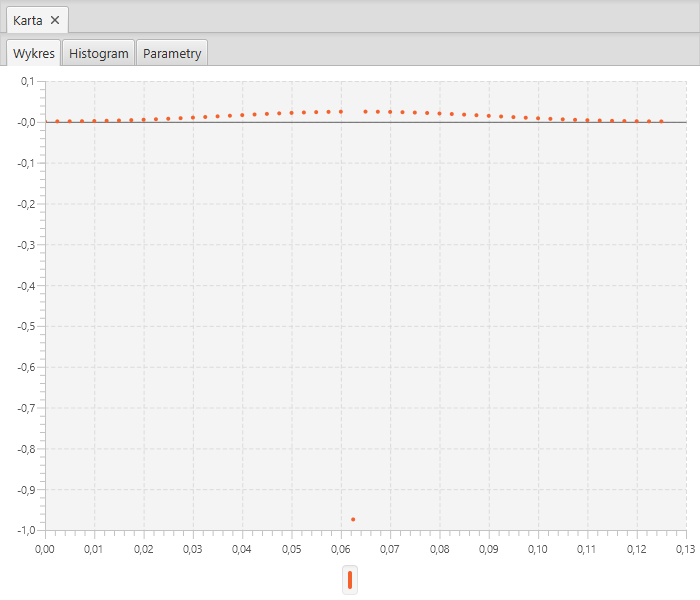
\includegraphics[width=0.6\textwidth]{img/result/filter/experiment11/data_draw_3d_filter_data_114210.png}
                \caption{Wykres filtra}
                \end{figure}

                \begin{figure}[H]
                \centering
                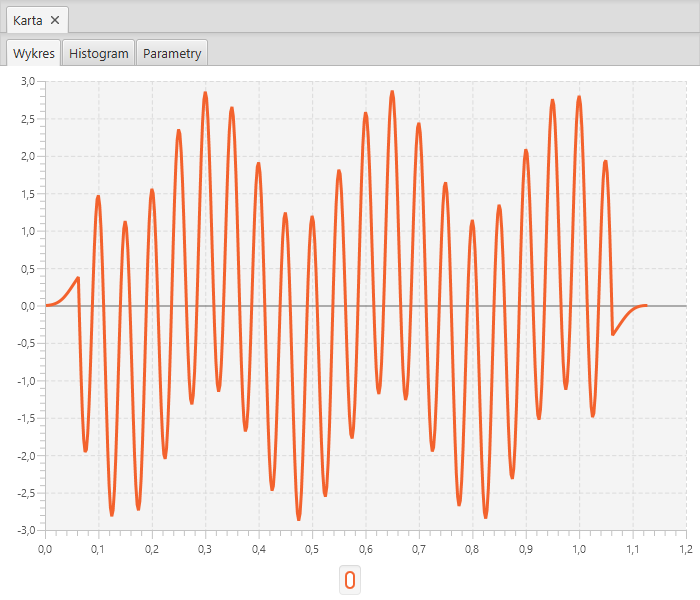
\includegraphics[width=0.6\textwidth]{img/result/filter/experiment11/data_draw_3d_result_reconstr_data_114319.png}
                \caption{Wykres sygnału po filtracji}
                \end{figure}
            }
            \newpage

            \subsubsection{Eksperyment 12} {
                \begin{table}[H]
                \centering
                \begin{tabular}{|l|l|l|l|l|l|}
                \hline
                Typ filtra & Rząd filtra & Częstotliwość odciecia & Typ okna  \\\hline
                 band\_pass & 51 & 90 & hamming     \\\hline
                \end{tabular}
                \caption{Parametry filtra}
                \end{table}
                \begin{figure}[H]
                \centering
                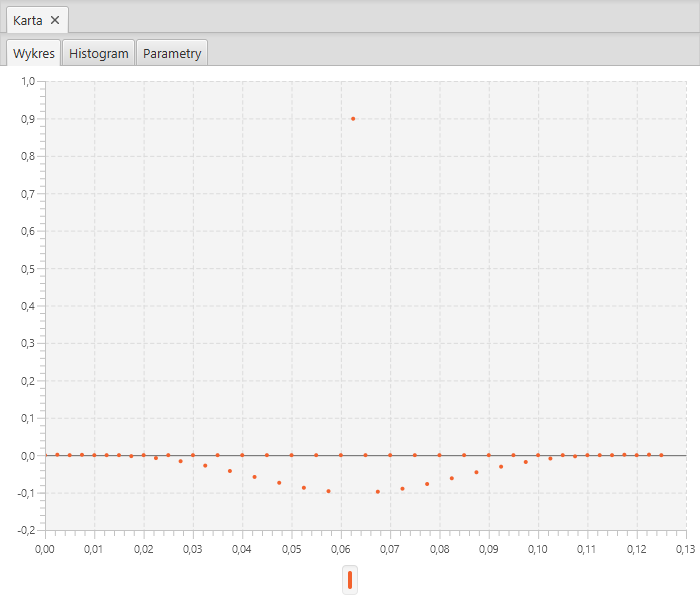
\includegraphics[width=0.6\textwidth]{img/result/filter/experiment12/data_draw_3e_filter_data_114327.png}
                \caption{Wykres filtra}
                \end{figure}

                \begin{figure}[H]
                \centering
                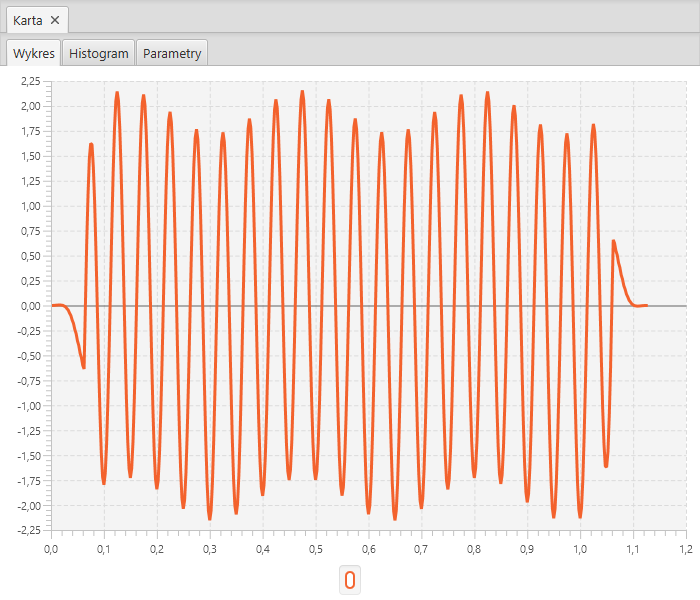
\includegraphics[width=0.6\textwidth]{img/result/filter/experiment12/data_draw_3e_result_reconstr_data_114439.png}
                \caption{Wykres sygnału po filtracji}
                \end{figure}
            }
            \newpage

            \subsubsection{Eksperyment 13} {
                \begin{table}[H]
                \centering
                \begin{tabular}{|l|l|l|l|l|l|}
                \hline
                Typ filtra & Rząd filtra & Częstotliwość odciecia & Typ okna  \\\hline
                band\_pass & 51 & 80 & hamming     \\\hline
                \end{tabular}
                \caption{Parametry filtra}
                \end{table}
                \begin{figure}[H]
                \centering
                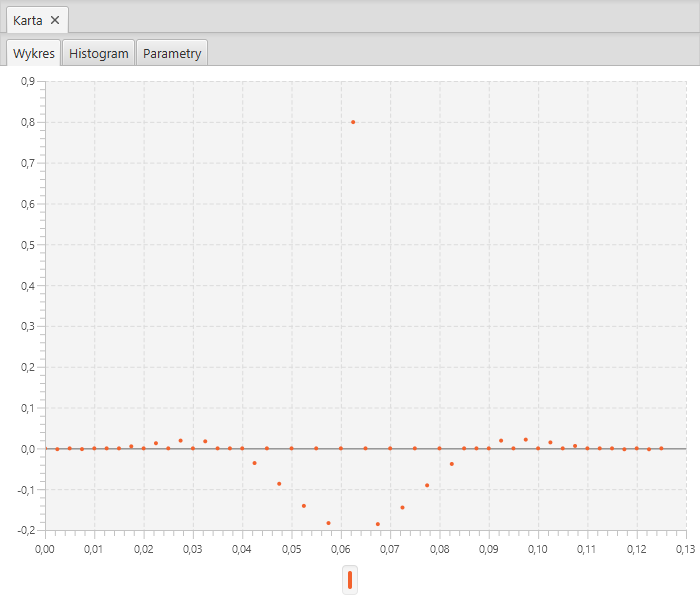
\includegraphics[width=0.6\textwidth]{img/result/filter/experiment13/data_draw_3f_filter_data_114446.png}
                \caption{Wykres filtra}
                \end{figure}

                \begin{figure}[H]
                \centering
                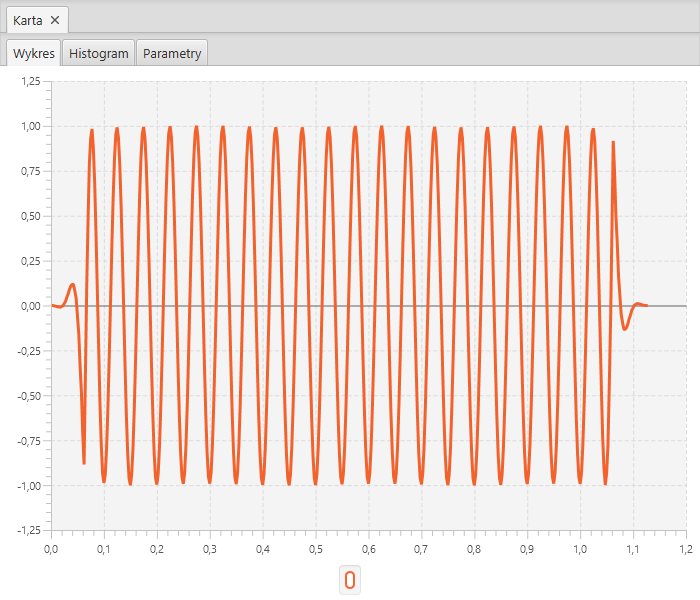
\includegraphics[width=0.6\textwidth]{img/result/filter/experiment13/data_draw_3f_result_reconstr_data_114550.png}
                \caption{Wykres sygnału po filtracji}
                \end{figure}
            }
            \newpage
        }

        \subsection{Wykorzystanie analizy korelacyjnej do pomiaru odległości} {

            \subsubsection{Eksperyment 1} {
                \begin{table}[H]
                    \centering
                    \begin{tabular}{|l|l|l|l|l|}
                        \hline
                        $V_s[m/s]$ & $V_p[m/s]$ & $T_s[s]$ & $f_s[Hz]$ & $l$ \\ \hline
                        100        & 0.5        & 1        & 20        & 60 \\ \hline
                    \end{tabular}
                    \caption{Parametry wejściowe symulatora}
                \end{table}
                \begin{figure}[H]
                    \centering
                    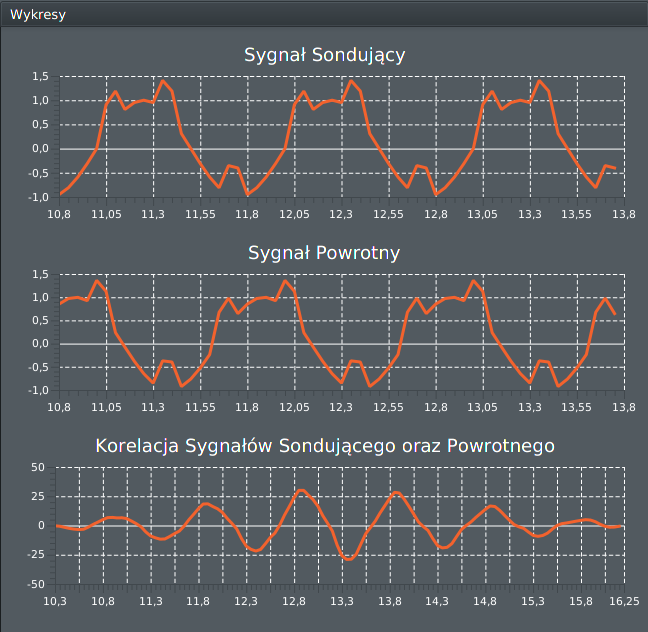
\includegraphics[width=0.8\textwidth]{img/result/simulation/experiment1.png}
                    \caption{Sygnały w symulatorze czujnika odległości}
                \end{figure}
                \begin{table}[H]
                    \centering
                    \begin{tabular}{|l|l|l|}
                        \hline
                        $t[s]$ & $d_r[m]$ & $d_m[m]$ \\ \hline
                        06.70  & 28.35    & 27.50    \\ \hline
                        09.70  & 29.85    & 30.00    \\ \hline
                        12.20  & 31.10    & 30.00    \\ \hline
                        17.10  & 33.55    & 32.50    \\ \hline
                    \end{tabular}
                    \caption{Wyniki działania symulatora}
                \end{table}
            }
            \newpage

            \subsubsection{Eksperyment 2} {
                \begin{table}[H]
                    \centering
                    \begin{tabular}{|l|l|l|l|l|}
                        \hline
                        $V_s[m/s]$ & $V_p[m/s]$ & $T_s[s]$ & $f_s[Hz]$ & $l$ \\ \hline
                        1000       & 0.5        & 0.1      & 200       & 40 \\ \hline
                    \end{tabular}
                    \caption{Parametry wejściowe symulatora}
                \end{table}
                \begin{figure}[H]
                    \centering
                    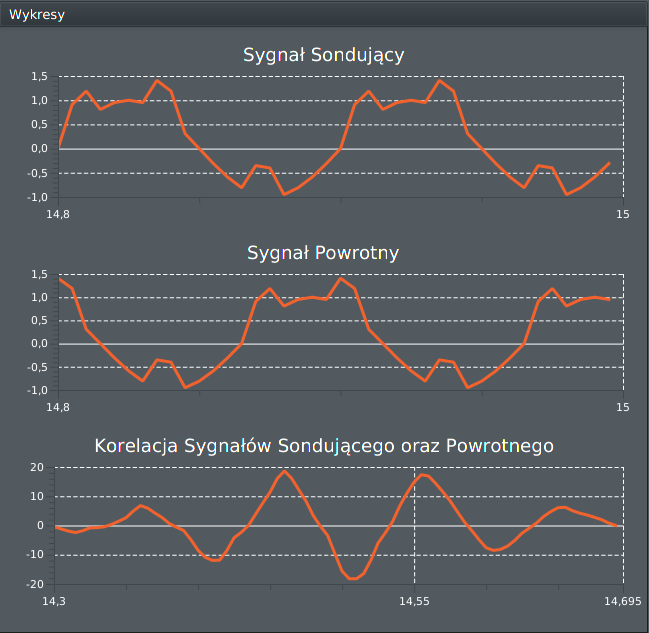
\includegraphics[width=0.8\textwidth]{img/result/simulation/experiment2.png}
                    \caption{Sygnały w symulatorze czujnika odległości}
                \end{figure}
                \begin{table}[H]
                    \centering
                    \begin{tabular}{|l|l|l|}
                        \hline
                        $t[s]$ & $d_r[m]$ & $d_m[m]$ \\ \hline
                        01.50  & 25.75    & 25.00    \\ \hline
                        02.90  & 26.45    & 27.50    \\ \hline
                        06.60  & 28.30    & 27.50    \\ \hline
                        15.00  & 32.50    & 30.00    \\ \hline
                    \end{tabular}
                    \caption{Wyniki działania symulatora}
                \end{table}
            }
            \newpage

            \subsubsection{Eksperyment 3} {
                \begin{table}[H]
                    \centering
                    \begin{tabular}{|l|l|l|l|l|}
                        \hline
                        $V_s[m/s]$ & $V_p[m/s]$ & $T_s[s]$ & $f_s[Hz]$ & $l$ \\ \hline
                        1000       & 0.5        & 0.1      & 400       & 40 \\ \hline
                    \end{tabular}
                    \caption{Parametry wejściowe symulatora}
                \end{table}
                \begin{figure}[H]
                    \centering
                    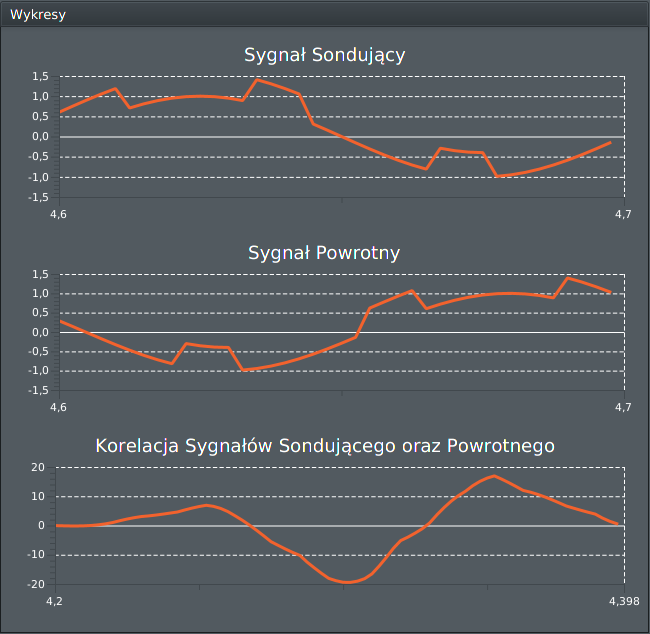
\includegraphics[width=0.8\textwidth]{img/result/simulation/experiment3.png}
                    \caption{Sygnały w symulatorze czujnika odległości}
                \end{figure}
                \begin{table}[H]
                    \centering
                    \begin{tabular}{|l|l|l|}
                        \hline
                        $t[s]$ & $d_r[m]$ & $d_m[m]$ \\ \hline
                        01.30  & 26.65    & 25.00    \\ \hline
                        03.10  & 26.55    & 26.25    \\ \hline
                        06.80  & 28.40    & 27.50    \\ \hline
                        08.50  & 29.25    & 28.75    \\ \hline
                    \end{tabular}
                    \caption{Wyniki działania symulatora}
                \end{table}
            }
            \newpage

            \subsubsection{Eksperyment 4} {
                \begin{table}[H]
                    \centering
                    \begin{tabular}{|l|l|l|l|l|}
                        \hline
                        $V_s[m/s]$ & $V_p[m/s]$ & $T_s[s]$ & $f_s[Hz]$ & $l$ \\ \hline
                        1000       & 0.5        & 0.1      & 400       & 20 \\ \hline
                    \end{tabular}
                    \caption{Parametry wejściowe symulatora}
                \end{table}
                \begin{figure}[H]
                    \centering
                    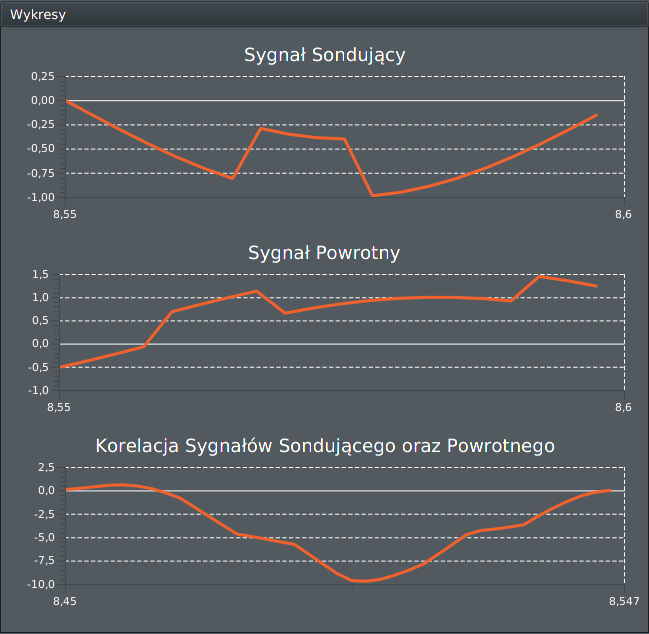
\includegraphics[width=0.8\textwidth]{img/result/simulation/experiment4.png}
                    \caption{Sygnały w symulatorze czujnika odległości}
                \end{figure}
                \begin{table}[H]
                    \centering
                    \begin{tabular}{|l|l|l|}
                        \hline
                        $t[s]$ & $d_r[m]$ & $d_m[m]$ \\ \hline
                        01.70  & 25.85    & 23.75    \\ \hline
                        03.50  & 26.75    & 23.75    \\ \hline
                        05.90  & 27.95    & 23.75    \\ \hline
                        08.60  & 29.30    & 23.75    \\ \hline
                    \end{tabular}
                    \caption{Wyniki działania symulatora}
                \end{table}
            }
            \newpage

            \subsubsection{Eksperyment 5} {
                \begin{table}[H]
                    \centering
                    \begin{tabular}{|l|l|l|l|l|}
                        \hline
                        $V_s[m/s]$ & $V_p[m/s]$ & $T_s[s]$ & $f_s[Hz]$ & $l$ \\ \hline
                        100        & 3.0        & 1        & 20        & 20 \\ \hline
                    \end{tabular}
                    \caption{Parametry wejściowe symulatora}
                \end{table}
                \begin{figure}[H]
                    \centering
                    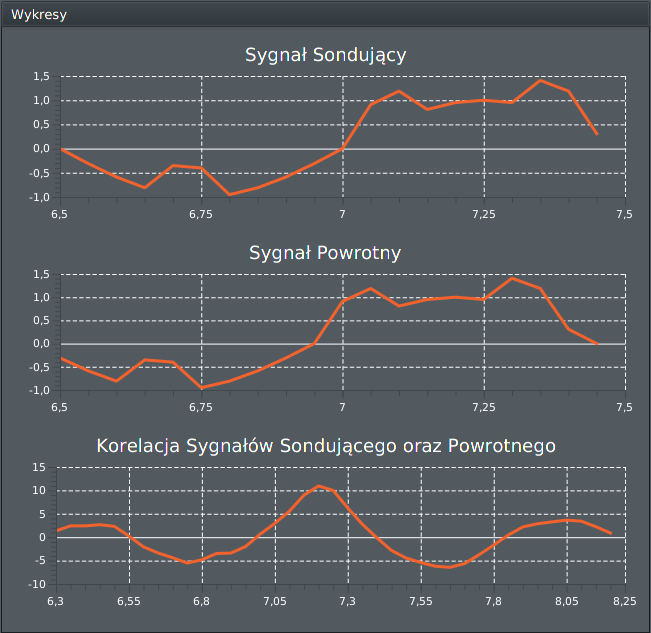
\includegraphics[width=0.8\textwidth]{img/result/simulation/experiment5.png}
                    \caption{Sygnały w symulatorze czujnika odległości}
                \end{figure}
                \begin{table}[H]
                    \centering
                    \begin{tabular}{|l|l|l|}
                        \hline
                        $t[s]$ & $d_r[m]$ & $d_m[m]$ \\ \hline
                        01.20  & 28.60    & 27.50    \\ \hline
                        03.10  & 34.30    & 32.50    \\ \hline
                        03.70  & 36.10    & 35.00    \\ \hline
                        04.40  & 38.20    & 37.50    \\ \hline
                        10.10  & 55.30    & 02.50    \\ \hline
                    \end{tabular}
                    \caption{Wyniki działania symulatora}
                \end{table}
            }
            \newpage

        }
    }
%--------------------------------------------------------------------------------------%
    \section{Dyskusja i wnioski} {

        \subsection{Splot i korelacja sygnałów dyskretnych} {
            Pierwsza wykonana seria eksperymentów jest poświęcona operacji splotu i
            korelacji sygnałów dykretnych, które to operacje należało zaimplementować w
            ramach wykonywanego zadania. Eksperymenty od \ref{eksperyment:splot1} do
            \ref{eksperyment:splot3} prezentują wyniki operacji splotu, a eksperymenty od
            \ref{eksperyment:korelacja1} do \ref{eksperyment:korelacja3} wyniki operacji
            korelacji. Dokumentacja każdego pojedynczego doświadczenia zawiera wykresy
            oraz parametry dwóch sygnałów na których operacja została wykonana, a także
            wykres sygnału wynikowego. W pierwszym doświadczenie \ref{eksperyment:splot1}
            wykorzystano dwa praktycznie takie same sygnały sinusoidalne, różniące się
            jedynie momentem rozpoczęcia, który to parametr nie ma wpływu na wynik
            splotu. Można więc uznać że wykonano splot dwóch takich samych sygnałów
            sinusoidalnych. Symetryczny kształt sygnału wynikowego wskazuje na to, że
            rzeczywiście sygnały wejścioweg były takie same. Ciekawe okazuje się
            porównanie z wynikami doświadczenia \ref{eksperyment:korelacja1}, w którym to
            te same sygnały zostały ze sobą skorelowane. Wynik tego eksperymenty jest
            odbiciem lustrzanym eksperymenty \ref{eksperyment:splot1} względem osi czasu,
            co wskazuje na pewne podobieństwo i związek między operacją splotu i korelacji
            sygnałów. W doświadczeniach \ref{eksperyment:splot2} i
            \ref{eksperyment:korelacja2} wykorzystano parę funkcji sinus i sinus
            wyprostowany jednopołówkowo. Wynik okazuje się w obu doświadczeniach bardzo
            podobny. Tym razem jednak odkrywamy, że jest to odbicie symetryczne nie tylko
            względem osi poziomej, ale również osi pionowej, czego ze względu na symetrię
            wykresu nie dało się zauważyć w poprzednio omawianej parze doświadczeń. W
            ostatniej parze eksperymentów \ref{eksperyment:splot3} oraz
            \ref{eksperyment:korelacja3} wykorzystano połączenie funkcji sinus z funkcją
            trójkątną. Wynik jest wizualnie ciekawy, w stosunku do wyników poprzednich.
            Okazuje się praktycznie identyczny dla splotu i korelacji ze względu na to,
            iż jest symetryczny względem swojego środka.
        }

        \subsection{Filtracja sygnałów dyskretnych} {
            Druga grupa eksperymentów poświęcona jest filtrom o skończonej odpowiedzi
            impulsowej. Na początku wygenerowany został sygnał przeznaczony do filtrowania,
            jak opisano w \ref{metody:filtracja}. Następnie w każdym kolejnym eksperymencie
            utworzony został nowy filtr, na którym wykonano splot ze wspomnianym wcześniej
            sygnałem złożonym. Dla każdego doświadczenia zaprezentowano wykres i parametry
            filtru oraz wykres sygnału po filtracji. Warto jeszcze przed analizą wyników
            zauważyć, że filtrowany sygnał posiada dwie, dające się wizualnie wyróżnić
            składowe, jedna o częstotliwości $20Hz$ a druga o częstotliwości $3Hz$.

            Pierwsze cztery eksperymenty poświęcone są badaniu wpływu wybranej funkcji
            okna na jakość filtracji. Tak więc kolejno zastosowane zostały okno
            kwadratowe, okno hamminga, okno hanninga i okno blackmana. W każdym przypadku
            wykorzystanu tutaj filtr dolnoprzepustowy rzędu 51 i częstotliwość odcięcia
            $5Hz$. Doświadczalnie stwierdzono, że przy tych parametrach różnica w
            wykorzystaniu okien staje się widoczna. I tak dla wspomnianych parametrów
            wizualnie daje się stwierdzić, że najlepszą jakość filtracji osiągnięto dla
            okna hammina, a najgorszą dla okna kwadratowego. Przy czym wyniki dla okna
            hanninga i hamminga niewiele się różnią, przy oknie blackmana daje się
            zauważyć, że jakaś inna częstotliwość składowa kiedyś istniała. Natomiast w
            przypadku okna prostokątnego składowa o wyższej częstotliwości wyraźnie się
            zaznacza. Warto jednak wspomnieć, że w każdym przypadku udało się tą wyższą
            składową wyraźnie lub całkowicie wytłumić.

            Kolejne trzy eksperymenty pokazują wpływ rzędu filtra (liczby jego próbek) na
            jakość filtrowania. Każdorazowo wykorzystano tutaj również filtr
            dolnoprzepustowy, czestotliwość odcięcia $5Hz$ i okno hammina. Wyniki okazują
            się zgodne z intuicją. Czym większy rząd filtra tym silniej udaje się wytłumić
            częstotliwość $20Hz$. Za pierwszym razem (rząd 41) wyższa składowa wytłumiona
            zostaje praktycznie całkowicie. Za drugim razem jest wyraźnie zauważalna, choć
            słabsza niż w sygnale oryginalnym. Wynik trzeciego doświadczenia (rząd 21)
            wizualnie niewiele różni się od sygnału filtrowanego.

            W ostatniej serii doświadczeń (od 8 do 13) wykorzystane zostały różne
            częstotliwości odcięcia jak i różne typy filtrów. W eksperymentach 8 i 9
            zastosowano częstotliwość odcięcia mniejszą i równą najniższej częstotliwości
            składowej sygnału, przy wykorzystaniu filtru dolnoprzepustowego. W wyniku
            wyższa składowa została wytłumiona całkowicie a niższa odpowiednio dla wyższej
            częstotliwości odcięcia - wytłumiona słabiej, natomiast dla niższej
            częstotliwości odcięcia - wytłumiona silniej. W ostatnich czterech
            doświadczeniach sygnał wynikowy został zrekonstruowany za pomocą interpolacji
            pierwszego rzędu w celu zwiększenia przejrzystości. Odfiltrowywana była bowiem
            czestotliwośc niższa, a pozostawiona częstotliwość wyższa - $20Hz$. W
            eksperymencie 10 zastosowano filtr górnoprzepustowy a częstotliwość odcięcia
            $f_o$ wynosiła 190, co dla tego filtru przekłada się na częstotliwość $f_{o2} =
            200Hz / 2 - 190Hz = 10Hz$. Na wykresie wynikowym widać, że faktycznie
            częstotliwość $3Hz$ została prawie całkowicie wytłumiona, da się jednak
            zauważyć jej obecność w nieznacznych "wahaniach" całego wykresu w góre i w
            dół. Przy zastosowaniu częstotliwości odcięcia $f_o = 195Hz$ dla tego samego
            filtra, wspomniana niższa częstotliwość zaznacza się znacznie wyraźniej. W obu
            przypadkach można jednak spokojnie stwierdzić, że składowa niższa jest
            słabsza niż składowa wyższa. Ostatnie dwa eksperymenty wykonano za pomocą
            filtra pasmowoprzepustowego, ustawiono częstotliwość odcięcia $f_o = 90Hz$, co
            dla tego filtra oznacza, że pasmo przepustowe mieściło się między $10Hz$ a
            $190$ Hz. W pierwszym z dwóch eksperymentów niższa częstotliwość została
            prawie całkowicie wytłumiona. W ostatnim przypadku częstotliwość niższa
            została wytłumiona tak, że nie jest już zauważalna na wykresie.
        }

        \subsection{Wykorzystanie analizy korelacyjnej do pomiaru odległości} {
            Ostatnia część eksperymentów została poświęcona badaniu zachowania
            korelacyjnego czujnika odległości. Dla każdego eksperymentu zostały
            przedstawione parametry wejściowe symulatora, wykresy sygnałów sondującego,
            powrotnego i ich korelacji oraz kilka pomiarów czujnika razem z rzeczywistymi
            odległościami. Pierwszy eksperyment został przeprowadzony dla prędkości
            sygnału $100m/s$ i odległości do przedmiotu około $30m$. Przedmiot oddala się
            nieznacznie z prędkością $0.5m/s$. Okres sygnału sondującego wynosi $1s$.
            Próbek w buforze jest $60$, co przy częstotliwości próbkowania $20Hz$ oznacza
            trzy pełne okresy. Okaże się, czy jest potrzeba przechowywać tyle próbek. Po
            przyjrzeniu się wynikom widać, że najogólniej mówiąc czujnik działa poprawnie,
            natomiast ma ograniczoną dokładność pomiaru do ok $2.5m$. Dokładność ta może
            być zadowalająca lub nie, w zależności od wymagań czujnika.

            \paragraph{Zakres działania czujnika} jest pierwszą rzeczą, na którą warto
            zwrócić uwagę. Można zastanowić się co ma na ten zakres decydujący wpływ.
            Rozważmy prędkość sygnału. Kolejny eksperyment (2) pokazuje, że sama prędkość
            nie wpływa w żaden sposób na dokładność pomiaru, gdyż przy prędkości $1000m/s$
            uzyskaliśmy tę samą dokładność, co przy prędkości $100m/s$. Ważny jest
            natomiast stosunek prędkości do okresu sygnału. Okres sygnału sondującego
            wyznacza zakres opóźnień, sygnału powrotnego, dla których uda się poprawnie
            obliczyć odległość. W idealnym przypadku, opóźnienie musi być oczywiście
            mniejsze niż okres, bo przy analizie korelacyjnej nie będzie się dało w żaden
            sposób stwierdzić, czy sygnał powrotny jest opóźniony o $kT + x$, czy tylko o
            $x$, gdzie $kT$ to dowolna całkowita wieloktrotność okresu a $x$ to pewne
            opóźnienie sygnału. W praktyce granica ta zależy od jeszcze wielu innych
            czynnników, jak charakterystyka samego sygnału sondującego oraz liczba okresów
            sygnału przechowywana w buforze. W eksperymencie 5 okazało się, że już gdy
            opóźnienie stało się większe niż ok $0.4$ część okresu, to czujnik nie był w
            stanie określić faktycznej odległości i zaczął znowu "od zera". Ostateczny
            wniosek jest więc taki, że na zakres działania czujnika ma wpływ stosunek
            prędkości sygnału sondującego do jego okresu. Sam okres wyznacza zakres
            opóźnień a prędkość decyduje o tym, jaki zakres odległości będzie odpowiadał
            danemu zakresowi opóźnień.

            \paragraph{Dokładność działania czujnika} zależy w decydującej mierze od
            częstotliwości próbkowania. A dokładnie nie od samej bezwzględnej wartości
            częstotliwości ale od liczby próbek przypadającej na okres. Czym więcej próbek
            na okres tym z większą dokładnością można stwierdzić, jakie jest opóźnienie
            sygnału powrotnego. Eksperyment 3 pokazuje, że po zwiększeniu częstotliwości
            próbkowania (co skutkowało zwiększeniem liczby próbek przypadających na okres
            sygnału), uzyskalismy większą dokładność niż w eksperymencie 2. Zostaje
            jeszcze do rozważenia ostatni parametr, a mianowicie długość bufora, którą od
            razu możemy przełożyć na faktycznie mającą znaczenie - liczbę okresów sygnału
            w buforze. Wartość ta jest bardzo istotna i eksperyment 4 pokazuje, że jeżeli
            będzie zbyt mała, to po prostu czujnik przestanie działać, gdyż analiza
            korelacyjna nie wykaże żadnego lokalnego maksimum korelacji. Pojawia się
            pytanie jaka powinna być wartość tego parametru. Oczywiście chcielibyśmy, żeby
            była jak najmniejsza, ponieważ czym mniej próbek w buforze, tym szybciej można
            przeprowadzić obliczenia, a czym szybciej znajdujemy wynik korelacji tym
            większą częstotliwość próbkowania możemy uzyskać, co w konsekwencji skutkuje
            większą dokładnością czujnika. W eksperymentach 1, 2 i 3 kolejno wartość ta
            była zmniejszana od trzykrotności okresu do pojedynczego okresu sygnału
            sondującego. Za żadnym razem zmniejszenie tej wartości nie wpłynęło negatywnie
            na analizę korelacyjną. Można więc na podstawie doświadczeń stwierdzić, że
            wystarczy w buforze przechowywać jeden okres. Okazuje się jednak, że nie jest
            to zasada, gdyż przy zastosowaniu mniej złożonej funkcji (np. czysty sinus),
            wartość ta była już za mała (niestety nie udokumentowano tego w tym
            sprawozdaniu). Można więc wysnuć wniosek, że charakter funkcji sondującej
            jest bardzo istotny, ponieważ od kształtu tej funkcji zależy, jaką minimalną
            wielokrotność (lub część) okresów trzeba przechować w buforze, aby poddana
            analizie korelacyjnej dała poprawne wyniki. Jak już wcześniej wspomniano, ma
            to decydujący wpływ na dokładność pomiaru.
        }
    }

    \section{Wnioski} {
        \begin{itemize}
            \item Operacje splotu i korelacji sygnałów dyskretnych są do siebie bardzo
                zbliżone
            \item Okno prostokątne najgorzej wpływa na jakość filtracji sygnału
            \item Czym większy rząd filtra tym lepsza jakość filtracji
            \item Jeżeli pasmo przepustowe nie obejmuje żadnej składowej to wszystkie
                składowe są tłumione, tym bardziej, im dalej znajdują się od granicy pasma
                przepustowego
            \item Korelacyjny czujnik odległości ma ograniczony zakres pomiaru wyznaczony
                przez stosunek prędkości sygnału sondującego do okresu tego sygnału
            \item Dokładność pomiaru korelacyjnego czujnika odległości jest zdeterminowana
                przez liczbę próbek przypadającą na jeden okres
            \item Charakterystyka sygnału sondującego ma duże znaczenie zarówno dla
                zakresu pomiaru czujnika korelacyjnego (charakterystyka wyniku korelacji),
                jak i dla dokładności pomiaru (minimalna długość bufora potrzebna do
                uzyskania poprawnego wyniku)
        \end{itemize}
    }

%--------------------------------------------------------------------------------------%

\end{document}
